\chapter{Research Outline}
In \autoref{ch:introduction}, some background on the difficulties of identification and cataloguing of NEAs was given. In this chapter, the resulting problem and associated knowledge gap will be presented. Then, the associated research questions and expected outcomes will be listed.

\section{Problem Statement}
Currently, humanity's knowledge of NEA populations is at a low level of completeness, especially for small diameter NEAs. Therefore, valuable scientific knowledge about the composition and evolution of the Solar system is unknown, and Earth is vulnerable to impacts which can be hazardous to human life and property. \\

It has been shown that current efforts are not adequate to reach the current goal of the spaceguard survey. Several missions have been proposed, and others are under development, which will cover this goal. However, a new more ambitious goal to identify smaller NEAs is still far out of reach. Even with a modern satellite positioned in deep space, only a limited survey completeness can be reached at limiting diameters $D < 100 \mathrm{m}$. This is caused by the limitations in position of this system, the required follow-up time and the number of detections required, and interference from the Sun.

\section{A Multi-Spacecraft Approach}
\label{sec:researchmultispacecraft}
To address this problem, we propose the option of a multi-spacecraft system. In recent years, spacecraft constellations have already shown a lot of potential in reaching complex mission goals. In the application of near-Earth asteroid surveys, more telescopes will firstly speed up the survey cadence, allowing the system to image the same area of sky at a faster rate. However, there are further synergystic advantages to such an approach. Three major benefits are noted in a multi-spacecraft system over a single telescope, which will be discussed in the following paragraphs.\\

Firstly, a multi-spacecraft system will mostly solve the problem of Solar glare: Although a spacecraft in syzygy with the Sun and an asteroid will not be able to detect the latter if it is located in the direction of the Sun, a different spacecraft located away from it might observe the Sun-asteroid arrangement from the side, allowing it to detect the target. In this way, a multi-spacecraft system is capable of minimizing the amount of blind spots in the search space. \autoref{fig:research_blind_spots} shows a visualisation of the reduction in blind areas when adding an additional spacecraft.\\

\begin{figure}[htbp]
 \centering
 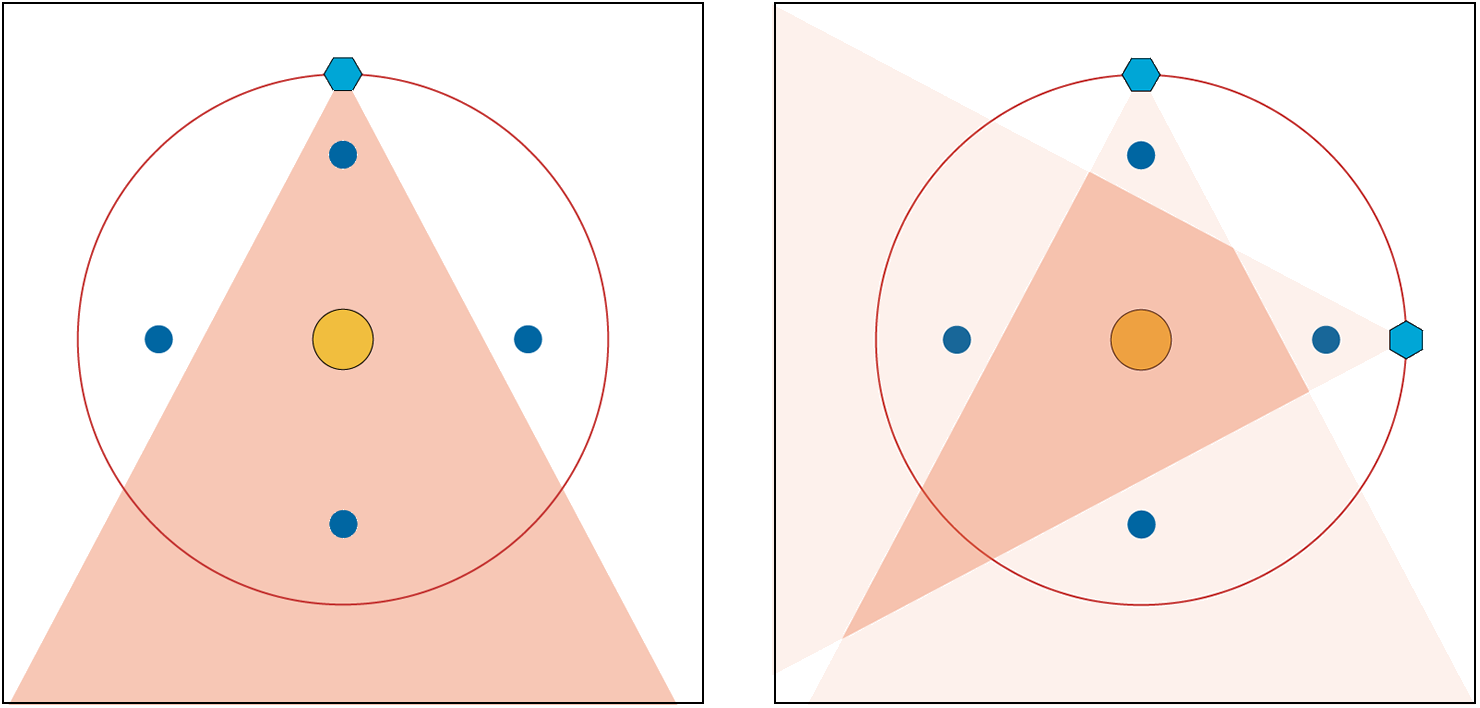
\includegraphics[width=0.8\textwidth]{img/research_blind_spots.png}
 \caption{Consider a spacecraft (represented by the cyan hexagon) attempting to observe several asteroids (blue circles). Because of Solar glare and thermal limits (red-shaded area), the spacecraft is unable to observe the top and bottom NEA. However, addition of a second spacecraft greatly reduces the ``blind area'': now the system can observe all four NEAs.}
 \label{fig:research_blind_spots}
\end{figure}


Secondly, using multiple spacecraft allows for easier identification and orbit determination of the NEA: Normally, a single telescope takes images in 2D of a target. As the asteroid will almost certainly be below the Rayleigh criterion of the telescope, it is not possible to estimate how close the asteroid is from its estimated diameter and the projected size on the sensor. Therefore, only the angular direction towards the target is known. Therefore, to obtain the orbit of the target requires solving Gauss' problem, which requires a minimum of three subsequent observations (six unknown parameters for the full orbit specification, two variables measured per observation). When using multiple spacecraft, it is possible to perform a kind of ``triangulation'', provided the spacecraft and the asteroid are not colinear. This allows for solving for the three-dimensional position of the asteroid. Thus, using only two observations in time reduces the orbit determination to Lambert's problem. This means the asteroid will only have to be within the area where telescopes can observe it for half the time as a single-spacecraft system. This is further shown in \autoref{fig:research_triangulation}, where addition of a second spacecraft allows for observing the asteroid before it moves out of the observable range.\\

\begin{figure}[htbp]
 \centering
 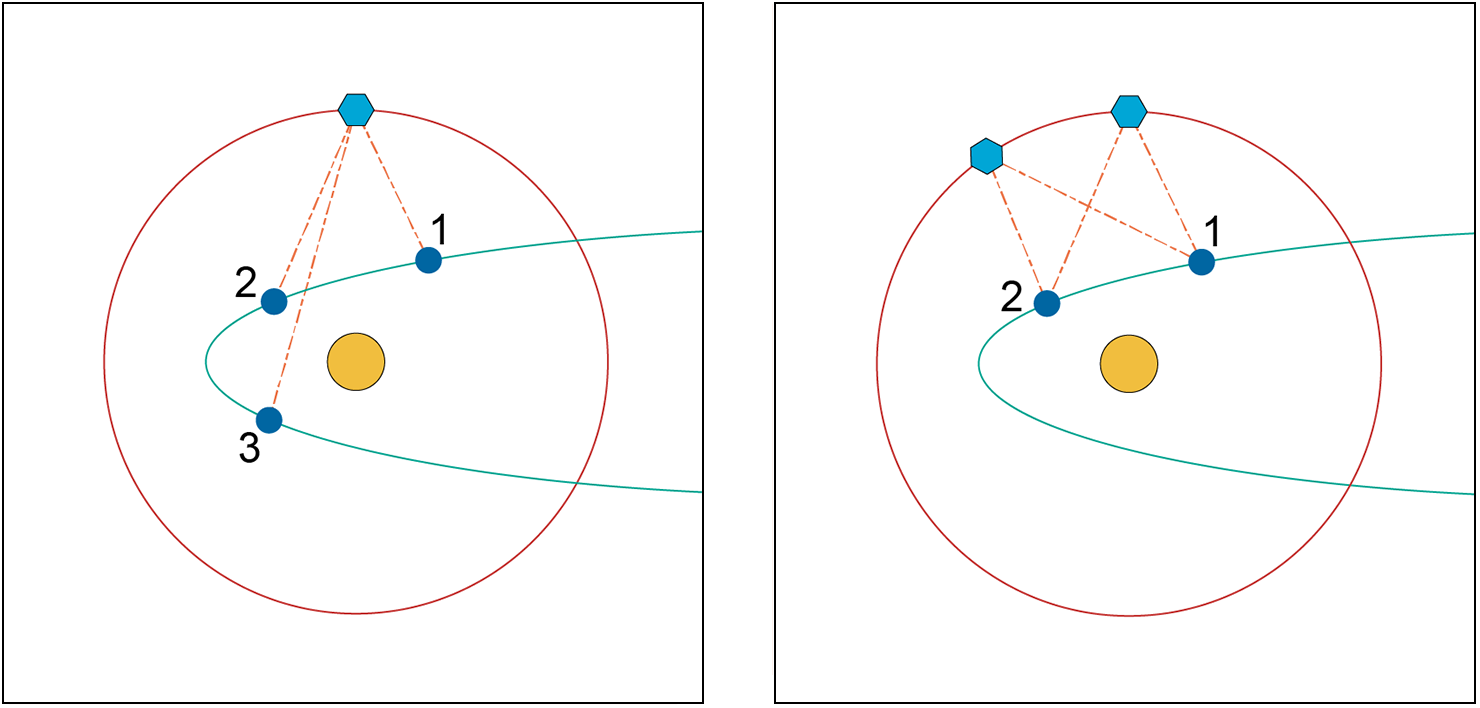
\includegraphics[width=0.8\textwidth]{img/research_triangulation.png}
 \caption{Normally, in order to perform orbit determination, the spacecraft (cyan hexagon) would have to image a target (blue cicle) three times. For targets that are hard to observe, such as a highly eccentric NEA which can only be detected close to perihelion, this leads to problems: the third detection will be hard to obtain, as the NEA moves behind the Sun into the blind area, or out of the detector's range altogether. Addition of a second spacecraft allows triangulation, thus halving the time required to identify the asteroid, performing the necessary measurements before the asteroid moves far away again.}
 \label{fig:research_triangulation}
\end{figure}


Lastly, a multi-spacecraft approach allows for more complex search strategies. The possibility for doing such search strategies when multiple sensors are available is demonstrated by the Cataline Sky Survey. Using their follow-up telescope, a new target is quickly selected for follow-up imaging, quickly gathering the required observations to perform orbit determination and thereby identification. In space, such a strategy would of course by more complex, as the problem becomes influenced by the location of the spacecraft. However, such an implementation will be very helpful in detecting NEAs which are only visible for a short period of time, such as highly eccentric objects with long semi-major axis, which are only visible for a short window around their perihelion. This idea is demonstrated in \autoref{fig:research_search_strategy}.\\

\begin{figure}[htbp]
 \centering
 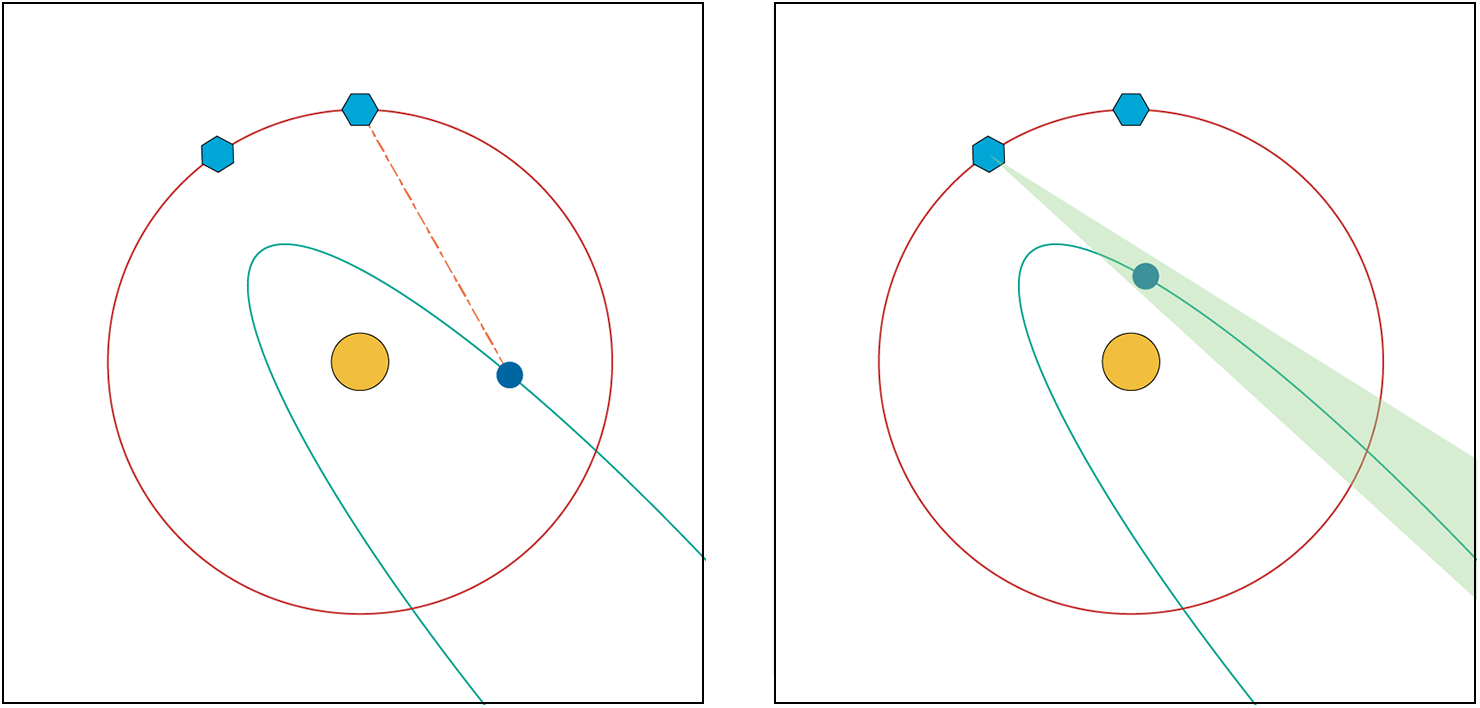
\includegraphics[width=0.8\textwidth]{img/research_search_strategy.png}
 \caption{In a more advanced system, some of the spacecraft could be dedicated to follow-up observations. As soon as one spacecraft detects a target, the second spacecraft is instructed to point in the direction of the new observation. In that way, even if a target is only observable for a short period, the spacecraft will have a much larger chance of pointing towards it.}
 \label{fig:research_search_strategy}
\end{figure}


However, before such strategies can be developed and implemented in a mission, it is first required to know the location and composition of such a multi-spacecraft system. To the author's best knowledge, the behavior of a multi-spacecraft survey has never been evaluated. In addition, to adequately assess the performance, it is vital to discover where the craft in such a system should be positioned, and how they should be equipped. The aim of this work are to provide insight into these points using simulation of such a survey.

\section{Research Questions and Expected Outcomes}
\label{sec:researchquestions}

To translate the aim into a concrete research topic, a main research question and a set of derived subquestions is composed. The main research question is:

\begin{center}\large\textbf{What is the optimal position and composition for a system of spacecraft with the purpose of identifying and cataloguing previously unidentified near-Earth asteroids?}\end{center}

A few terms deserve special attention: To begin, the terms \textit{position and composition} serve to indicate the scope of the research. As mentioned previously, no previous work has been published on multi-spacecraft NEA surveys. The current body of work on space-based surveys commonly uses general categories of orbits such as Venus-trailing orbits, or orbits at Lagrange points. In addition, either thermal infrared or a visual light telescope is used. In a multi-spacecraft system, the position should be treated in a more general sense: there is the added element of combining different positions synergistically, as explained in the previous section. Also, the composition with regards to payload is worthy of investigation: perhaps, a synergistic combination of slower but more sensitive infrared and faster but less sensitive visual light telescopes might be of merit. In addition to specifying what should be researched, these terms also limit the scope: other aspects, including - but not limited to - search strategy, communication between spacecraft, and image processing techniques will be left to further research. \\

The second factor of note is \textit{identifying and cataloguing}. The distinction between observation, detection, identification and cataloguing is worth the discourse before continuing. Essentially, these terms all represent successive steps in the survey. An \textit{observation} is when a target is within the telescope's field of view when an image is taken. Of course, this is not useful in and of itself. Therefore, a \textit{detection} can be established when the signal-to-noise ratio of the asteroid in the image is sufficiently high. At this point, it is clear that ``something'' is present in the telescope's field of view. When enough detections are established within a certain time frame, it becomes possible to determine the orbit of the target, and to see whether or not it is already known. At this point, an \textit{identification} can be performed from the subsequent observations. Then, with the orbit of the target known, the survey can proceed to \textit{cataloguing} the NEA by transmitting the relevant data back to Earth for analysis and storage. Thus, it is apparent that just observing or detecting an NEA is not useful in and of itself. For the information to be relevant, the system should be capable of assisting in the identification and cataloguing efforts. \\

The last term important to give some discourse to before further explaining the research is \textit{unidentified} asteroids. As was discussed in \autoref{sec:introductionidentification}, humanity has already catalogued a sizeable portion of the NEA population. Of course, it is not neccessary to identify these targets again. Therefore, the research effort should be concentrated on solving the identified problem of improving the knowledge of the small-diameter NEA population. \\

In support of the main research question, in conjunction with the aim of addressing the problem through a numerical simulation, several subquestions were drafted to assist in providing an answer. The first three subquestions are related to the design of the simulation; how to accurately produce and operate a model of NEA surveys. The next three questions are related to the parameters of such missions; where the spacecraft are located and how the system is composed. Lastly, a subquestion is included which will be essential for judging the results in the context of current and future endeavors, such as those listed in \autoref{sec:introductionidentification} and \autoref{sec:introductionproposals}. The subquestions are explained in brief below:
\begin{enumerate}
 \item \textbf{How can the population of NEAs be accurately modelled, and how can these models be adjusted for unidentified NEA's?}: The first subquestion is related to simulation. As mentioned above, the model needs to give an accurate estimate for how the system will perform in surveying unidentified NEA's. Therefore, first a model of this population is required. Although this may seem straightforward, it might pose some challenges: after all, only the identified portion of the NEA population is known, the unidentified portion is clearly not. Fortunately, literature sources are available to assist in this process.
 \item \textbf{How can surveys of NEA's by a system of spacecraft be accurately modelled?}: Having the asteroid population, the next consideration is how to model a survey of that population. Again, good sources in literature are available to assist in solving this question, although sufficient verification and validation will need to be performed.
 \item \textbf{How can the position and composition of the system be optimized?}: Already mentioned above, the possibilities for positioning and composing a multi-spacecraft system grow exponentially with the number of spacecraft in the system. Therefore, a good method of optimizing the system is required. It is expected that the simulation will be computationally expensive, and possibly noisy. Therefore, selection of a proper optimization method is crucial to ensure good results.
 \item \textbf{What is the effect of increasing the number of spacecraft on the process and performance of identifying and cataloguing NEA's?}: The first question related to the behavior of the system, and probably the most straightforward relation to consider when looking at the research question. Although it is apparent that an increase in the number of spacecraft will always increase the performance (or at worst, have it stay constant), the number of spacecraft is the most relevant free parameter to have results on, as it is a very important concept to explore and consider for future missions.
 \item \textbf{How is the performance of possible payload compositions affected by the number of spacecraft, and what is the resulting optimal payload composition?}: Secondly, the payload of the system. As explained in \autoref{sec:introductionproposals}, current research often uses either a visual or a thermal infrared telescope. However, when considering a multi-spacecraft system, combinations of these are possible. It will be good to see which of the systems benefits mostly from the increase in the number of spacecraft, and whether synergistic effects occur in ``hybrid'' systems composed of a mix of instrumentation. 
 \item \textbf{How do the number of spacecraft and payload interact with the orbital parameters of the system?}: The last of the free parameters, the positioning of the spacecraft. Although it is not very crucial for the preliminary stage of mission design which is the target of this mission, it is important to understand what the interaction between these factors is and how this affects the performance.
 \item \textbf{How effective is a system of multiple spacecraft at identifying and cataloguing previously unidentified NEA's compoared to other current and future methods?}: A multi-spacecraft survey mission is a very costly endeavor, requiring several expensive spacecraft and vehicles for launching these into outer space. Although this work will not go into detail on the economics of space missions, a realistic assessment to the merits of the idea should be made to consider whether it would be worth it to develop such a mission. 
\end{enumerate}

It is expected that through answering this research question, several outcomes will be obtained. The main goal is to provide outcomes which are useful in doing further research into, as well as designing, future NEA survey missions. The desired outcomes of this work are thus as follows:
\begin{enumerate}
 \item Understanding how increasing the number of spacecraft affects the performance of a NEA system. Of course, the performance will increase, however the main interest is in how much this performance increases, and thus whether such a solution is worth considering for future missions. It is expected that in addition to this, insight will be gained into any diminishing returns for higher numbers of spacecraft, and perhaps limits beyond which adding addition spacecraft provides no tangible benefit anymore.
 \item A conclusion on where to focus efforts with regards to payload. Currently, thermal infrared telescopes are considered the best choice for future NEA missions (e.g. \cite{2017NEOSDT}, \cite{ThesisOlga}). However, perhaps the benefits of a multi-spacecraft system are expressed stronger in a visual light system, or a hybrid system might provide a synergistic benefit.
 \item Insight into changes to the optimal orbital position for the spacecraft as a function of the number of spacecraft. It is expected that these quantities will undergo some change, and mapping this out allows for relating the results to the results of other studies on where to position NEA survey spacecraft.
 \item Reliable estimated for what performance to expect as a higher number of spacecraft is utilized in the system. In addition, this result is also interesting is reverse: seeing what kind of system would be necessary to obtain a desired result provides a basis for designing a mission out of such a requirement.
\end{enumerate}

Through fulfilling these goals and providing the expected outcomes, a useful base for further work on these kind of NEA surveys will thus be laid. 
